\documentclass[border=0pt]{standalone}
\newcommand{\revlamina}{6}
\providecommand{\revlamina}{1}
% Preámbulo común de las láminas FV (A3 horizontal, 420 x 297 mm)
\usepackage[T1]{fontenc}
\usepackage[utf8]{inputenc}
\usepackage[spanish,es-nodecimaldot]{babel}
\usepackage[scaled=0.92]{helvet}
\renewcommand{\familydefault}{\sfdefault}
\usepackage{tikz}
\usetikzlibrary{arrows.meta,patterns,calc,babel,positioning}
\usepackage{siunitx}
\sisetup{output-decimal-marker={,},mode=text}
\DeclareSIUnit\kWp{kWp}
\DeclareSIUnit\ohm{\ensuremath{\Omega}}

\definecolor{inv1}{RGB}{37,99,180}
\definecolor{inv2}{RGB}{22,128,84}
\definecolor{nfpa}{RGB}{200,30,30}
\definecolor{viento}{RGB}{40,70,200}
\definecolor{sombra}{RGB}{230,130,0}
\definecolor{losa}{RGB}{120,190,200}
\definecolor{dc}{RGB}{225,95,0}
\definecolor{exist}{RGB}{110,110,110}
\definecolor{nuevo}{RGB}{190,20,20}

% Marcador de referencia numerada
\newcommand{\refm}[2]{\node[circle,draw=black,fill=white,line width=0.35pt,inner sep=0pt,minimum size=3.4mm,font=\fontsize{5.5}{6}\selectfont\bfseries] at #1 {#2};}

% Cajetín: \cajetin{lamina}{titulo}{contenido}{escala}{hoja}
\newcommand{\cajetin}[5]{%
  \draw[line width=0.6pt] (250,10) rectangle (410,58);
  \draw[line width=0.3pt] (250,46) -- (410,46);
  \draw[line width=0.3pt] (250,34) -- (410,34);
  \draw[line width=0.3pt] (250,22) -- (410,22);
  \draw[line width=0.3pt] (370,10) -- (370,34);
  \draw[line width=0.3pt] (330,10) -- (330,22);
  \node[anchor=north west,font=\fontsize{6}{7}\selectfont,align=left] at (251.5,57) {\textbf{Instituto Tecnológico de Costa Rica} -- EL-4601 Normalización Técnica para Electrónica\\Proyecto No.~2: Diseño normativo de una instalación solar fotovoltaica};
  \node[anchor=north west,font=\fontsize{6}{7}\selectfont,align=left] at (251.5,45) {\textbf{Proyecto:} Sistema FV 20,88~kWp -- Edificio Centro Académico de Alajuela (TEC)\\\textbf{Propietario:} Universidad Técnica Nacional -- Catastro A-652521-2000};
  \node[anchor=north west,font=\fontsize{6.5}{7.5}\selectfont,align=left,text width=115mm] at (251.5,33) {\textbf{Contenido:} #2\\#3};
  \node[anchor=north west,font=\fontsize{5.5}{6.5}\selectfont,align=left] at (371.5,33) {\textbf{Lámina}};
  \node[font=\fontsize{16}{18}\selectfont\bfseries] at (390,25.5) {#1};
  \node[anchor=north west,font=\fontsize{5.5}{6.5}\selectfont,align=left] at (251.5,21) {\textbf{Elaboró:} Grupo de trabajo EL-4601\\\textbf{Revisó:} \rule{25mm}{0.2pt}\\\textbf{Fecha:} 7/10/2026 \quad \textbf{Rev.:} \revlamina};
  \node[anchor=north west,font=\fontsize{5.5}{6.5}\selectfont,align=left] at (331.5,21) {\textbf{Escala (A3):}\\#4};
  \node[anchor=north west,font=\fontsize{5.5}{6.5}\selectfont,align=left] at (371.5,21) {\textbf{Hoja:}\\#5};
}
% Marco de la lámina
\newcommand{\marco}{%
  \draw[line width=0.2pt,white] (0,0) rectangle (420,297);
  \draw[line width=0.8pt] (10,10) rectangle (410,287);
}

\begin{document}
\begin{tikzpicture}[x=1mm,y=1mm]
\marco
\node[anchor=north west,inner sep=0pt] at (15,283) {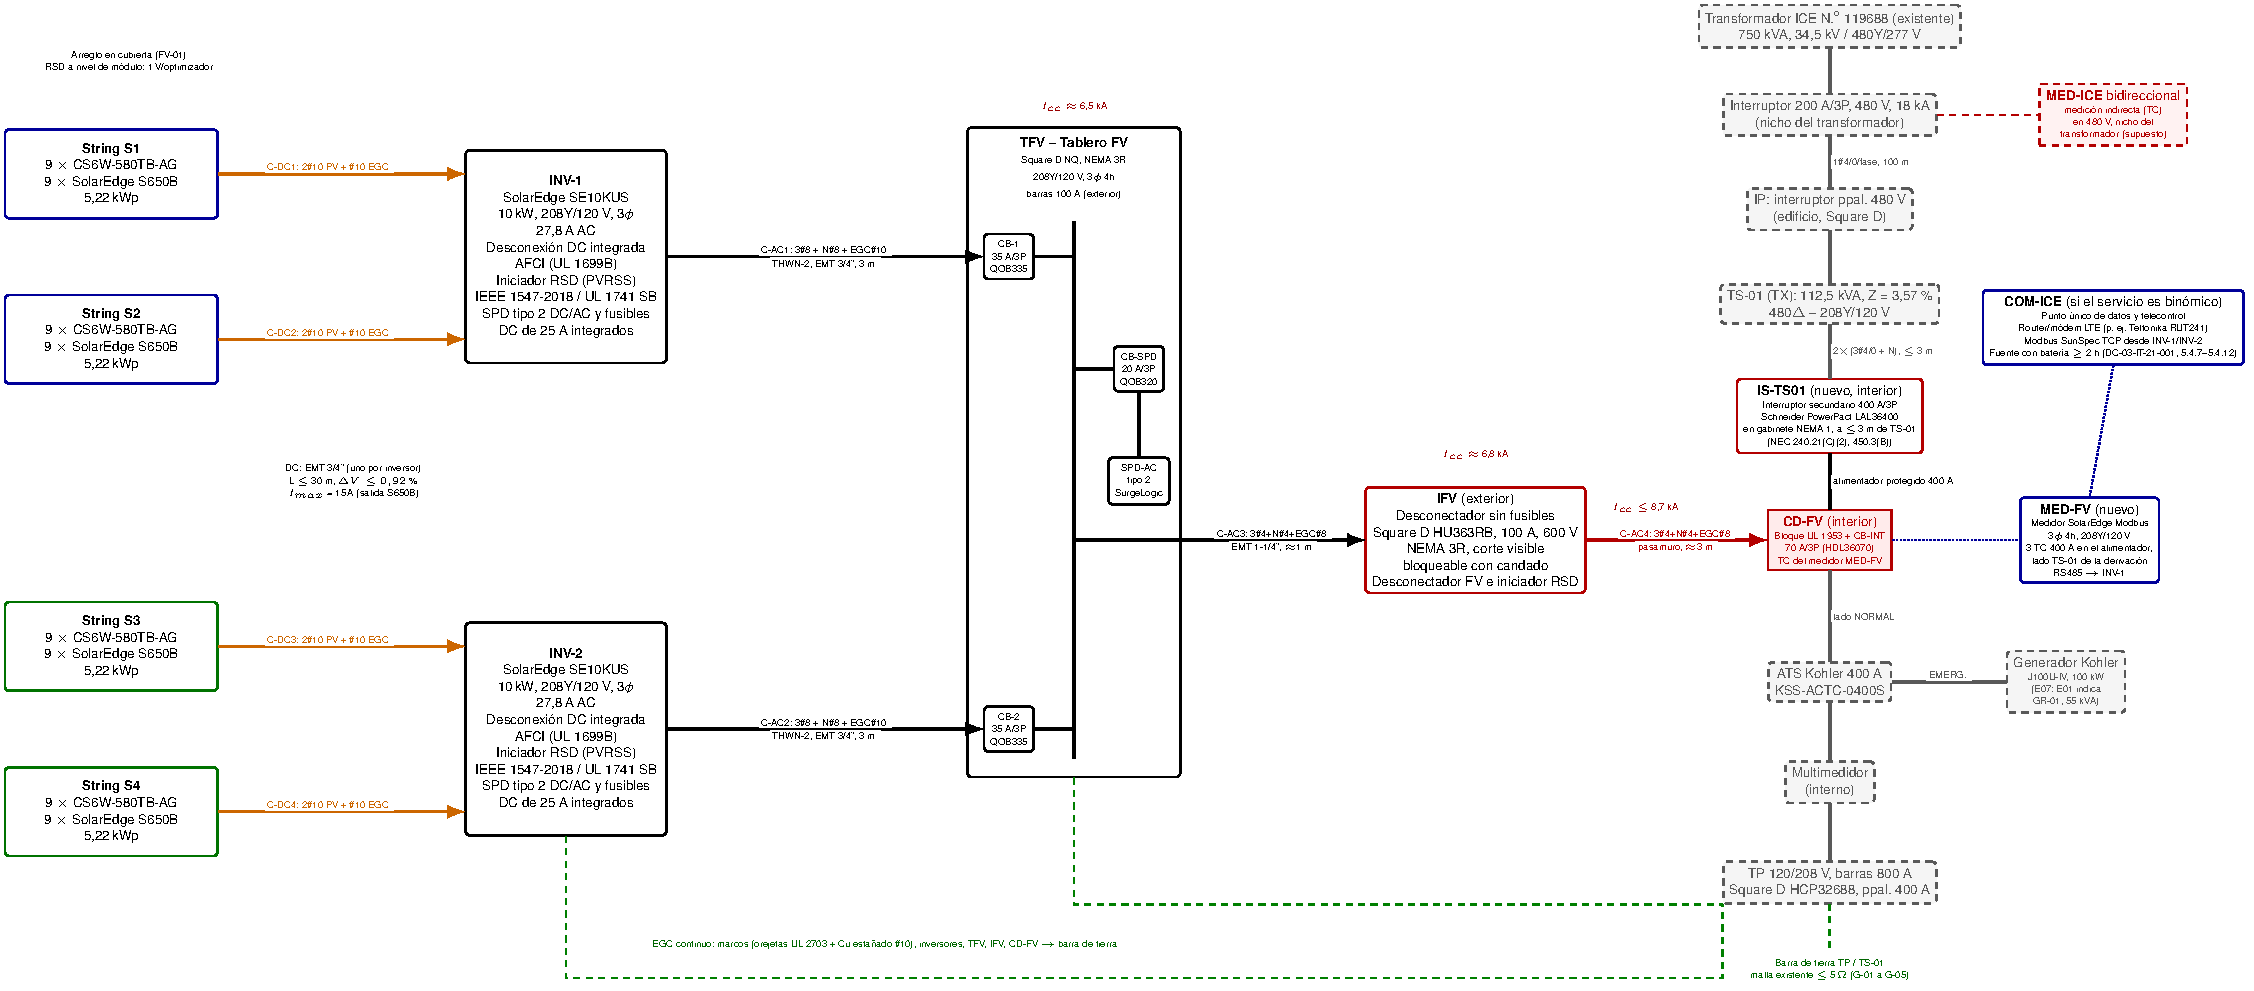
\includegraphics[width=390mm]{unifilar_fv_sa.pdf}};
\node[anchor=north west,font=\fontsize{10}{12}\selectfont\bfseries] at (15,66) {DIAGRAMA UNIFILAR COMPLETO DEL SISTEMA FV E INTERCONEXIÓN};
\node[anchor=north west,font=\fontsize{6.2}{7.6}\selectfont,align=left,text width=228mm] at (15,59) {%
\textbf{Notas}\\
1. Interconexión en el alimentador TS-01 $\rightarrow$ ATS (lado NORMAL). Si falla la red del ICE, los inversores cesan la inyección en $\le$ 2 s (IEEE 1547-2018) antes de que el ATS transfiera; el generador nunca queda en paralelo con el sistema FV. Ajuste del controlador MPAC 1200: retardo de detección de falla de la fuente normal $\ge$ 3 s.\\
2. Nuevo interruptor secundario IS-TS01 de 400 A a $\le$ 3 m de TS-01 (NEC 240.21(C)(2); 450.3(B): 400 A es el valor normalizado siguiente al 125 \% de 312,3 A). El tramo IS-TS01 $\rightarrow$ ATS pasa a ser un alimentador protegido en su origen: 2 $\times$ \#4/0 = 460 A $\ge$ 400 A (NEC 705.12(B)(2)(1)(b), con el principal de 400 A del TP aguas abajo).\\
3. Derivación del alimentador protegido: conductor \#4 (79,9 A corregidos) $\ge$ (400 + 1,25 $\times$ 55,6)/10 = 47,0 A y $\ge$ 70 A de CB-INT, terminada a $\le$ 3 m en CB-INT dentro de CD-FV (NEC 240.21(B)(1) con 705.12(B)(2)(2)).\\
4. Un string por par de entradas del inversor; la salida de cada optimizador está limitada a 15 A, así que no se requieren fusibles de string externos (NEC 690.9(A)(1)). El SE10KUS integra fusibles DC de 25 A y SPD tipo 2 en DC y AC (ficha del fabricante).\\
5. Apagado rápido: al abrir el IFV (o CB-1/CB-2) los inversores pierden la red AC y cada S650B baja a 1 V (NEC 690.12).\\
6. Interruptores retroalimentados (QOB, HDL) atornillables y aptos para retroalimentación (NEC 705.12(D), (E)). Corriente de falla disponible (NEC 110.9, 110.24): $\le$ 8,7 kA en CD-FV, $\approx$ 6,8 kA en el IFV y $\approx$ 6,5 kA en el TFV; QOB 10 kA, HDL 25 kA a 240 V y SCCR del IFV $\ge$ 10 kA.\\
7. Elementos en gris punteado = existentes (as-built E01, E07--E09), con los datos de placa verificados en sitio el 5/10/2026.\\
8. Inversores: categoría B del ICE por defecto (DC-03-IT-21-001, 5.7.2), modo volt-var activo por defecto (5.7.6) y ajustes finales según indique el ICE para el punto de acople común. Si el servicio es binómico, COM-ICE da el punto único de datos y telecontrol (5.4.7--5.4.12). El ATS KSS (serie estándar) es de transición abierta.\\
9. MED-ICE: no aparece en los planos ni en el cuarto eléctrico. Supuesto de diseño: medición indirecta en 480 V en el nicho del transformador (E01); el ICE la sustituye por un medidor bidireccional al firmar el contrato.\\
10. MED-FV: los 3 TC se instalan en el alimentador entre TS-01 y la derivación, abrazando los 2 conductores en paralelo de cada fase, para medir el intercambio neto con la red.};
% Leyenda
\node[anchor=north west,font=\fontsize{9}{11}\selectfont\bfseries] at (252,104) {LEYENDA};
\begin{scope}[shift={(252,92)},font=\fontsize{6}{7.4}\selectfont]
\draw[very thick,orange!80!black] (0,6) -- (12,6); \node[anchor=west] at (14,6) {Circuito DC (PV Wire en EMT)};
\draw[very thick] (0,1) -- (12,1); \node[anchor=west] at (14,1) {Circuito AC nuevo (THWN-2 en EMT)};
\draw[very thick,gray!70!black] (0,-4) -- (12,-4); \node[anchor=west] at (14,-4) {Circuito existente};
\draw[thick,green!50!black,dashed] (0,-9) -- (12,-9); \node[anchor=west] at (14,-9) {Conductor de puesta a tierra de equipos (EGC)};
\draw[thick,blue!60!black,densely dotted] (0,-14) -- (12,-14); \node[anchor=west] at (14,-14) {Medición / comunicación};
\draw[thick,rounded corners=1pt] (80,4) rectangle (92,8); \node[anchor=west] at (94,6) {Equipo nuevo};
\draw[thick,dashed,gray!70!black,fill=gray!8,rounded corners=1pt] (80,-1) rectangle (92,3); \node[anchor=west] at (94,1) {Equipo existente};
\draw[thick,red!70!black,fill=red!8] (80,-6) rectangle (92,-2); \node[anchor=west] at (94,-4) {Punto de interconexión};
\draw[thick,dashed,red!70!black,fill=red!5] (80,-11) rectangle (92,-7); \node[anchor=west] at (94,-9) {Elemento supuesto (dato adoptado)};
\end{scope}
\cajetin{FV-03}{Diagrama unifilar completo: strings, inversores, tableros,}{protecciones, conductores e interconexión}{Sin escala}{4 de 5}
\end{tikzpicture}
\end{document}
